\section{Solution design}
We started with a system design step.
Regarding this, we realized sequence diagrams
that describe the sequences of interaction between the simple
frontend and the microservice-based backend. These also take
into account the communications that happen among different
microservices that are involved in the same use case. One example
is the restaurant reservation use case that passes
through an authentication microservice and another microservice
that handles the restaurants’ data. Here we describe the microservices
that we designed and attach the corresponding sequence diagrams showing
the interactions among them.

\subsection{Microservices}

\subsubsection{User auth}

The user auth microservice exposes an interface for authentication needs of the
user. These are mainly related to login and registration via the frontend web app
and identity validation via the backend for operations that need authentication.
The main idea is to have an API that responds to requests, by operating on a
NoSQL database. The database contains information about the users: Name, Surname,
Email address, Password, and Session Tokens. The user registers into the system
and a new entry in the database is created. When a user logs in, a new session
is created by generating a unique token. This token is stored in the database
and sent to the frontend to be cached. The system is purely RESTful and thus
stateless. Every request is authenticated via the auth token.\\
The available operations are:
\begin{itemize}
    \item Login (Figure \ref{fig:user_login}): The client provides email and
    password (or token) and receives a session token if the user is registered.
    \item Registration (Figure \ref{fig:user_registration}): The client provides name,
    surname, email and password, and receives a session token after being registered
    in the database. The operation fails if a user with the same email already exists.
    \item Logout: The current login session is canceled.
    \item Token validation: The calling microservice (the one that needs a request to
    be authenticated) provides the email and session token of the user that initiated
    the operation and receives a validation or an error, depending on the validity of
    the token. This operation is shown in Figure \ref{fig:reserve}.
\end{itemize}

\begin{figure}
    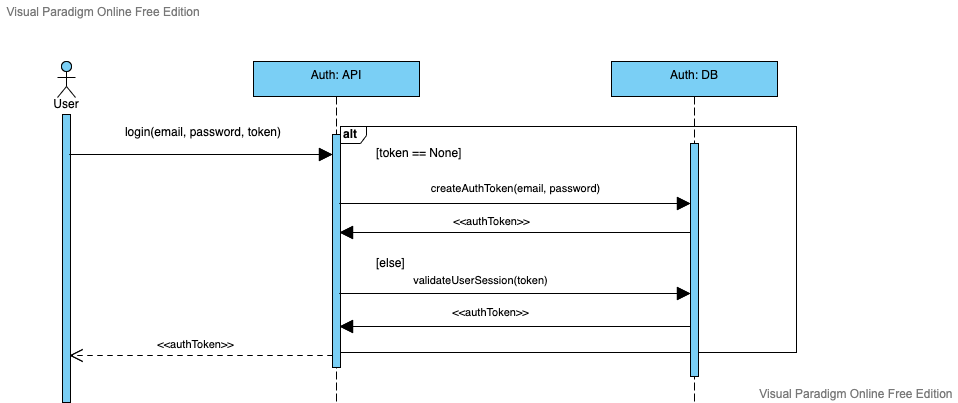
\includegraphics[width=\linewidth]{../docs/sequence/userAuth/auth.png}
    \caption{User login sequence diagram.}
    \label{fig:user_login}
\end{figure}

\begin{figure}
    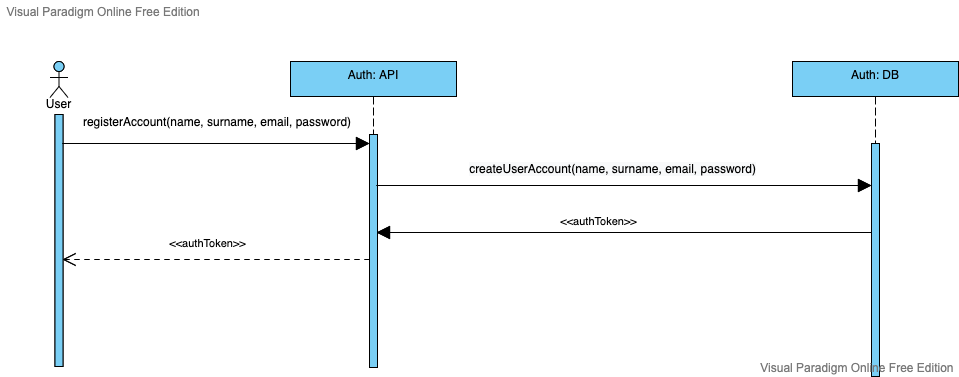
\includegraphics[width=\linewidth]{../docs/sequence/userRegistration/registerUser.png}
    \caption{User registration sequence diagram.}
    \label{fig:user_registration}
\end{figure}

\subsubsection{Restaurant auth}

The restaurant auth microservice exposes an interface for authentication needs of the
restaurant. It is very similar to the one of the user, but it is separated to better
divide contextes. In fact, the scalability needs of the two authentication services are
quite different. After the release of such a system, the increase in the number of users
is expected to be much more significant than the one of the number of registered
restaurants. This division guarantees individual scalability.
Also in this case there is an API that responds to requests, by operating on a
NoSQL database. The database contains authentication information about the restaurants:
Name, Email address, Password, and Session Tokens. The tokens work the same way they
do in the user auth module.\\
The available operations are:
\begin{itemize}
    \item Login (Figure \ref{fig:restaurant_login}): The client provides email and
    password (or token) and receives a session token if the user is registered.
    \item Logout: The current login session is canceled.
    \item Token validation: The calling microservice (the one that needs a request to
    be authenticated) provides the email and session token of the restaurant that initiated
    the operation and receives a validation or an error, depending on the validity of
    the token. This operation is shown in Figure \ref{fig:manage_booking}.
\end{itemize}

\begin{figure}
    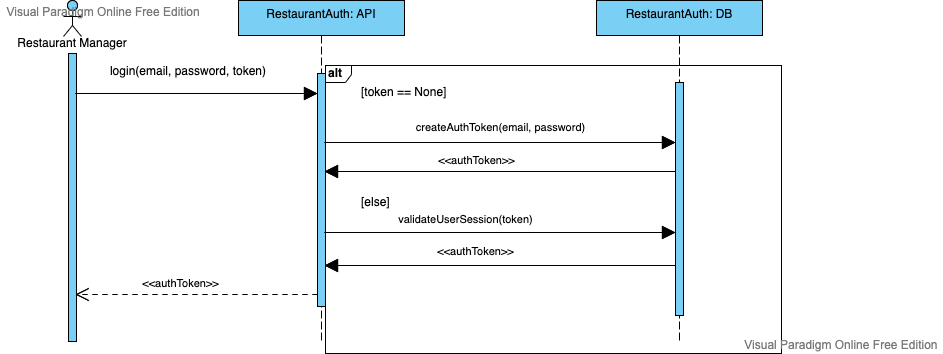
\includegraphics[width=\linewidth]{../docs/sequence/restaurantAuth/restaurantAuth.png}
    \caption{Restaurant login sequence diagram.}
    \label{fig:restaurant_login}
\end{figure}

\subsubsection{Restaurant data}

\begin{figure}
    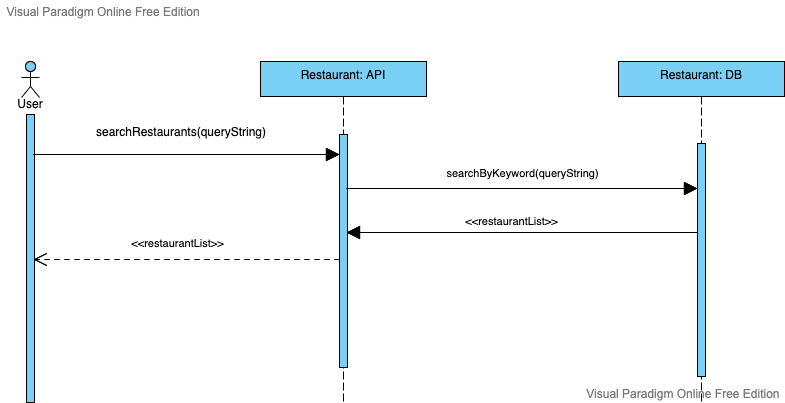
\includegraphics[width=\linewidth]{../docs/sequence/search/search.png}
    \caption{Restaurant search sequence diagram.}
    \label{fig:restaurant_search}
\end{figure}

\subsubsection{Booking}

Reservation (Figure \ref{fig:reserve})

\begin{figure}
    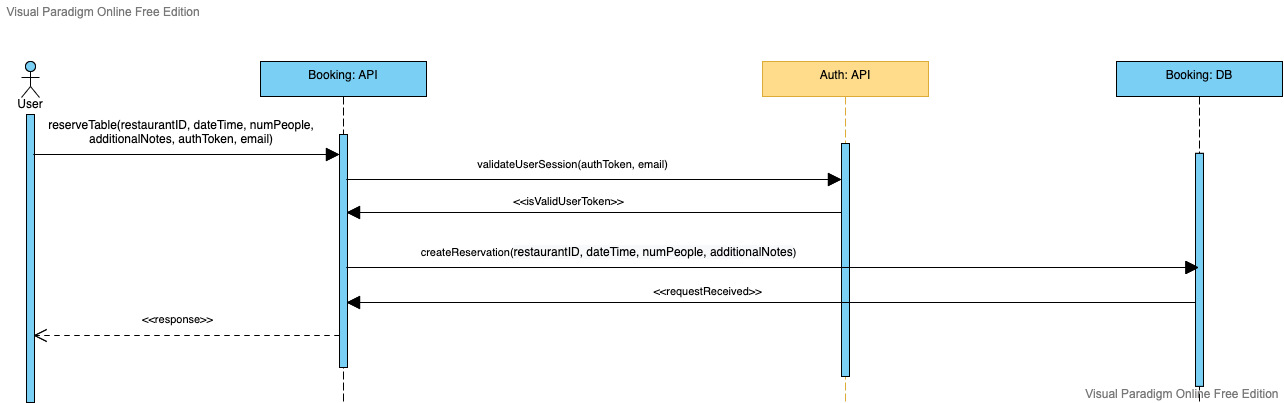
\includegraphics[width=\linewidth]{../docs/sequence/booking/reserve.png}
    \caption{Reservation sequence diagram.}
    \label{fig:reserve}
\end{figure}

\begin{figure}
    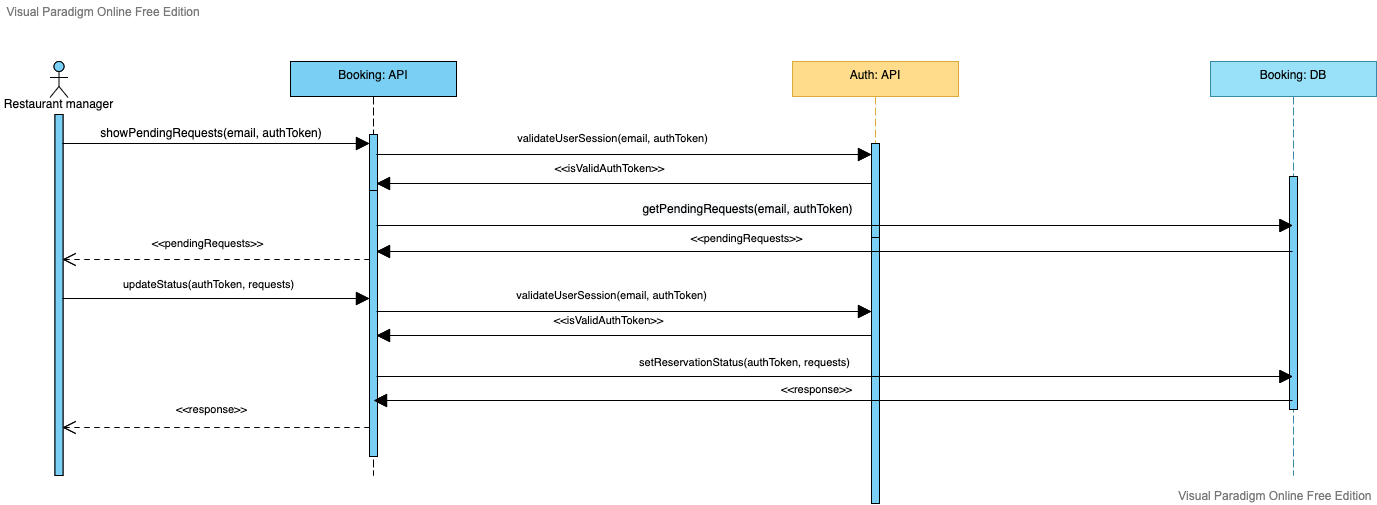
\includegraphics[width=\linewidth]{../docs/sequence/manageBooking/manageBooking.png}
    \caption{Booking management sequence diagram.}
    \label{fig:manage_booking}
\end{figure}

\subsection{Scalability}

By structuring the system into many microservices, there is the possibility
to scale the single microservices indipendently. This is useful since the
microservices may receive different loads of incoming traffic and this
way there is more control over which component should be scaled.